%==============================================================================
% tento soubor pouzijte jako zaklad
% this file should be used as a base for the thesis
% Autoři / Authors: 2008 Michal Bidlo, 2018 Jaroslav Dytrych
% Kontakt pro dotazy a připomínky: dytrych@fit.vutbr.cz
% Contact for questions and comments: dytrych@fit.vutbr.cz
%==============================================================================
% kodovani: UTF-8 (zmena prikazem iconv, recode nebo cstocs)
% encoding: UTF-8 (you can change it by command iconv, recode or cstocs)
%------------------------------------------------------------------------------
% zpracování / processing: make, make pdf, make clean
%==============================================================================
% Soubory, které je nutné upravit: / Files which have to be edited:
%   xdlaba02-Ztratova-komprese-plenoptickych-fotografii-20-literatura-bibliography.bib - literatura / bibliography
%   xdlaba02-Ztratova-komprese-plenoptickych-fotografii-01-kapitoly-chapters.tex - obsah práce / the thesis content
%   xdlaba02-Ztratova-komprese-plenoptickych-fotografii-30-prilohy-appendices.tex - přílohy / appendices
%==============================================================================
\documentclass[zadani]{fitthesis} % bez zadání - pro začátek práce, aby nebyl problém s překladem
%\documentclass[english]{fitthesis} % without assignment - for the work start to avoid compilation problem
%\documentclass[zadani]{fitthesis} % odevzdani do wisu a/nebo tisk s barevnými odkazy - odkazy jsou barevné
%\documentclass[english,zadani]{fitthesis} % for submission to the IS FIT and/or print with color links - links are color
%\documentclass[zadani,print]{fitthesis} % pro černobílý tisk - odkazy jsou černé
%\documentclass[english,zadani,print]{fitthesis} % for the black and white print - links are black
%\documentclass[zadani,cprint]{fitthesis} % pro barevný tisk - odkazy jsou černé, znak VUT barevný
%\documentclass[english,zadani,cprint]{fitthesis} % for the print - links are black, logo is color
% * Je-li práce psaná v anglickém jazyce, je zapotřebí u třídy použít
%   parametr english následovně:
%   If thesis is written in english, it is necessary to use
%   parameter english as follows:
%      \documentclass[english]{fitthesis}
% * Je-li práce psaná ve slovenském jazyce, je zapotřebí u třídy použít
%   parametr slovak následovně:
%   If the work is written in the Slovak language, it is necessary
%   to use parameter slovak as follows:
%      \documentclass[slovak]{fitthesis}
% * Je-li práce psaná v anglickém jazyce se slovenským abstraktem apod.,
%   je zapotřebí u třídy použít parametry english a enslovak následovně:
%   If the work is written in English with the Slovak abstract, etc.,
%   it is necessary to use parameters english and enslovak as follows:
%      \documentclass[english,enslovak]{fitthesis}

% Základní balíčky jsou dole v souboru šablony fitthesis.cls
% Basic packages are at the bottom of template file fitthesis.cls
% zde můžeme vložit vlastní balíčky / you can place own packages here

% Kompilace po částech (rychlejší, ale v náhledu nemusí být vše aktuální)
% Compilation piecewise (faster, but not all parts in preview will be up-to-date)
% \usepackage{subfiles}

% Nastavení cesty k obrázkům
% Setting of a path to the pictures
%\graphicspath{{obrazky-figures/}{./obrazky-figures/}}
%\graphicspath{{obrazky-figures/}{../obrazky-figures/}}

%---rm---------------
\renewcommand{\rmdefault}{lmr}%zavede Latin Modern Roman jako rm / set Latin Modern Roman as rm
%---sf---------------
\renewcommand{\sfdefault}{qhv}%zavede TeX Gyre Heros jako sf
%---tt------------
\renewcommand{\ttdefault}{lmtt}% zavede Latin Modern tt jako tt

% vypne funkci šablony, která automaticky nahrazuje uvozovky,
% aby nebyly prováděny nevhodné náhrady v popisech API apod.
% disables function of the template which replaces quotation marks
% to avoid unnecessary replacements in the API descriptions etc.
\csdoublequotesoff

% =======================================================================
% balíček "hyperref" vytváří klikací odkazy v pdf, pokud tedy použijeme pdflatex
% problém je, že balíček hyperref musí být uveden jako poslední, takže nemůže
% být v šabloně
% "hyperref" package create clickable links in pdf if you are using pdflatex.
% Problem is that this package have to be introduced as the last one so it
% can not be placed in the template file.
\ifWis
\ifx\pdfoutput\undefined % nejedeme pod pdflatexem / we are not using pdflatex
\else
  \usepackage{color}
  \usepackage[unicode,colorlinks,hyperindex,plainpages=false,pdftex]{hyperref}
  \definecolor{hrcolor-ref}{RGB}{223,52,30}
  \definecolor{hrcolor-cite}{HTML}{2F8F00}
  \definecolor{hrcolor-urls}{HTML}{092EAB}
  \hypersetup{
	linkcolor=hrcolor-ref,
	citecolor=hrcolor-cite,
	filecolor=magenta,
	urlcolor=hrcolor-urls
  }
  \def\pdfBorderAttrs{/Border [0 0 0] }  % bez okrajů kolem odkazů / without margins around links
  \pdfcompresslevel=9
\fi
\else % pro tisk budou odkazy, na které se dá klikat, černé / for the print clickable links will be black
\ifx\pdfoutput\undefined % nejedeme pod pdflatexem / we are not using pdflatex
\else
  \usepackage{color}
  \usepackage[unicode,colorlinks,hyperindex,plainpages=false,pdftex,urlcolor=black,linkcolor=black,citecolor=black]{hyperref}
  \definecolor{links}{rgb}{0,0,0}
  \definecolor{anchors}{rgb}{0,0,0}
  \def\AnchorColor{anchors}
  \def\LinkColor{links}
  \def\pdfBorderAttrs{/Border [0 0 0] } % bez okrajů kolem odkazů / without margins around links
  \pdfcompresslevel=9
\fi
\fi
% Řešení problému, kdy klikací odkazy na obrázky vedou za obrázek
% This solves the problems with links which leads after the picture
\usepackage[all]{hypcap}

% Informace o práci/projektu / Information about the thesis
%---------------------------------------------------------------------------
\projectinfo{
  %Prace / Thesis
  project={BP},            %typ práce BP/SP/DP/DR  / thesis type (SP = term project)
  year={2019},             % rok odevzdání / year of submission
  date=\today,             % datum odevzdání / submission date
  %Nazev prace / thesis title
  title.cs={Ztrátová komprese plenoptických fotografií},  % název práce v češtině či slovenštině (dle zadání) / thesis title in czech language (according to assignment)
  title.en={Lossy compression of light-filed photography}, % název práce v angličtině / thesis title in english
  %title.length={14.5cm}, % nastavení délky bloku s titulkem pro úpravu zalomení řádku (lze definovat zde nebo níže) / setting the length of a block with a thesis title for adjusting a line break (can be defined here or below)
  %Autor / Author
  author.name={Drahomír},   % jméno autora / author name
  author.surname={Dlabaja},   % příjmení autora / author surname
  %author.title.p={Bc.}, % titul před jménem (nepovinné) / title before the name (optional)
  %author.title.a={Ph.D.}, % titul za jménem (nepovinné) / title after the name (optional)
  %Ustav / Department
  department={UPGM}, % doplňte příslušnou zkratku dle ústavu na zadání: UPSY/UIFS/UITS/UPGM / fill in appropriate abbreviation of the department according to assignment: UPSY/UIFS/UITS/UPGM
  % Školitel / supervisor
  supervisor.name={David},   % jméno školitele / supervisor name
  supervisor.surname={Bařina},   % příjmení školitele / supervisor surname
  supervisor.title.p={Ing.},   %titul před jménem (nepovinné) / title before the name (optional)
  supervisor.title.a={Ph.D.},    %titul za jménem (nepovinné) / title after the name (optional)
  % Klíčová slova / keywords
  keywords.cs={Ztrátová komprese obrazu, světelné pole, plenoptická fotografie, JPEG, AVC, HEVC.}, % klíčová slova v českém či slovenském jazyce / keywords in czech or slovak language
  keywords.en={Lossy image compression, light field, plenoptic photography, JPEG, AVC, HEVC.}, % klíčová slova v anglickém jazyce / keywords in english
  %keywords.en={Here, individual keywords separated by commas will be written in English.},
  % Abstrakt / Abstract
  abstract.cs={
    Cílem této práce je vhodně navrhnout a implementoval ztrátový kodek pro plenoptické fotografie.
    První implementovanou procedurou pro kompresi je zrcadlení metody JPEG do tří a čtyř rozměrů, které jsou reprezentovány jednotlivými pohledy plenoptické fotografie.
    Dále jsou implementovány metody využívající ke kompresi plenoptické fotografie metody pro kompresi videa AVC a HEVC.
    Zrcadlením metody JPEG do čtyř rozměrů se povedlo při stejném PSNR dosáhnout kompresního poměru X:Y, což je oproti referenčnímu 2D JPEG kodeků zlepšení o ZZ\%.
    Využitím metod pro kompresi videa bylo dosaženo kompresního poměru X:Z.
    Z výsledků vyplývá, že je ze zkoumaných kodeků pro kompresi plenoptických fotografií nejvhodnější metoda YYY.},
    % abstrakt v českém či slovenském jazyce / abstract in czech or slovak language
  abstract.en={\todo{Přeložit kompletní abstrakt}}, % abstrakt v anglickém jazyce / abstract in english
  %abstract.en={An abstract of the work in English will be written in this paragraph.},
  % Prohlášení (u anglicky psané práce anglicky, u slovensky psané práce slovensky) / Declaration (for thesis in english should be in english)
  declaration={Prohlašuji, že jsem tuto bakalářskou práci vypracoval samostatně pod vedením\\
  Ing. Davida Bařiny, Ph.D.\\
  Uvedl jsem všechny literární prameny a publikace, ze kterých jsem čerpal.},
  %declaration={Hereby I declare that this bachelor's thesis was prepared as an original author’s work under the supervision of Mr. X
% The supplementary information was provided by Mr. Y
% All the relevant information sources, which were used during preparation of this thesis, are properly cited and included in the list of references.},
  % Poděkování (nepovinné, nejlépe v jazyce práce) / Acknowledgement (optional, ideally in the language of the thesis)
  acknowledgment={Rád bych poděkoval vedoucímu mé práce za poskytnutou odbornou pomoc.},
  %acknowledgment={Here it is possible to express thanks to the supervisor and to the people which provided professional help
%(external submitter, consultant, etc.).},
  % Rozšířený abstrakt (cca 3 normostrany) - lze definovat zde nebo níže / Extended abstract (approximately 3 standard pages) - can be defined here or below
  %extendedabstract={Do tohoto odstavce bude zapsán rozšířený výtah (abstrakt) práce v českém (slovenském) jazyce.},
  %faculty={FIT}, % FIT/FEKT/FSI/FA/FCH/FP/FAST/FAVU/USI/DEF
  faculty.cs={Fakulta informačních technologií}, % Fakulta v češtině - pro využití této položky výše zvolte fakultu DEF / Faculty in Czech - for use of this entry select DEF above
  faculty.en={Faculty of Information Technology}, % Fakulta v angličtině - pro využití této položky výše zvolte fakultu DEF / Faculty in English - for use of this entry select DEF above
  department.cs={Ústav matematiky}, % Ústav v češtině - pro využití této položky výše zvolte ústav DEF nebo jej zakomentujte / Department in Czech - for use of this entry select DEF above or comment it out
  department.en={Institute of Mathematics} % Ústav v angličtině - pro využití této položky výše zvolte ústav DEF nebo jej zakomentujte / Department in English - for use of this entry select DEF above or comment it out
}

% Rozšířený abstrakt (cca 3 normostrany) - lze definovat zde nebo výše / Extended abstract (approximately 3 standard pages) - can be defined here or above
%\extendedabstract{Do tohoto odstavce bude zapsán výtah (abstrakt) práce v českém (slovenském) jazyce.}

% nastavení délky bloku s titulkem pro úpravu zalomení řádku - lze definovat zde nebo výše / setting the length of a block with a thesis title for adjusting a line break - can be defined here or above
%\titlelength{14.5cm}


% řeší první/poslední řádek odstavce na předchozí/následující stránce
% solves first/last row of the paragraph on the previous/next page
\clubpenalty=10000
\widowpenalty=10000

% checklist
\newlist{checklist}{itemize}{1}
\setlist[checklist]{label=$\square$}

\begin{document}
  % Vysazeni titulnich stran / Typesetting of the title pages
  % ----------------------------------------------
  \maketitle
  % Obsah
  % ----------------------------------------------
  \setlength{\parskip}{0pt}

  {\hypersetup{hidelinks}\tableofcontents}

  % Seznam obrazku a tabulek (pokud prace obsahuje velke mnozstvi obrazku, tak se to hodi)
  % List of figures and list of tables (if the thesis contains a lot of pictures, it is good)
  \ifczech
    \renewcommand\listfigurename{Seznam obrázků}
  \fi
  \ifslovak
    \renewcommand\listfigurename{Zoznam obrázkov}
  \fi
  % \listoffigures

  \ifczech
    \renewcommand\listtablename{Seznam tabulek}
  \fi
  \ifslovak
    \renewcommand\listtablename{Zoznam tabuliek}
  \fi
  % \listoftables

  \ifODSAZ
    \setlength{\parskip}{0.5\bigskipamount}
  \else
    \setlength{\parskip}{0pt}
  \fi

  % vynechani stranky v oboustrannem rezimu
  % Skip the page in the two-sided mode
  \iftwoside
    \cleardoublepage
  \fi

  % Text prace / Thesis text
  % ----------------------------------------------
  %===============================================================================
% Autoři: Michal Bidlo, Bohuslav Křena, Jaroslav Dytrych, Petr Veigend a Adam Herout 2018

\chapter{Úvod}
S rozvojem nových technologií pro zachycení scény v prostoru a čase rostou také nároky na archivaci a přenos těchto scén po síti.
Příkladem takové technologie je plenoptická fotografie.
Dosud se jednalo spíše o experimentální odvětví počítačové grafiky patřící do výzkumných laboratoří, ale s nástupem výkonnějšího hardwaru se rozšiřuje i mezi širokou veřejnost.

Taková fotografie nese nejen informace o barvě, ale také o směru paprsku dopadajícího na světelný senzor.
Informace o směru paprsků vytváří mnohem kompletnější reprezentaci zachycené scény.
Z plenoptické fotografie lze například rekonstruovat pohled na scénu z jiného místa pozorování či s jiným zorným úhlem.
Lze tak například vytvořit ortografickou reprezentaci zachycené scény.
Také je možné softwarově měnit rovinu zaostření a simulovat různé velikosti clony.
To vše bez nutnosti převádět fotografii na point cloud či jiný trojrozměrný formát.

V praxi to ovšem znamená, že plenoptická fotografie oproti klasické fotografii klade mnohonásobně větší nároky na kapacitu paměti.
Plenoptické fotografie je proto potřeba efektivně komprimovat.
Jelikož je tato technologie poměrně dlouho známá a její rozšíření omezuje primárně nedostatečný hardwarový výkon, byla pro plenoptické fotografie vyvinuta řada kompresních metod, které jsou založeny na existujících algoritmech pro kompresi klasických fotografií, videa či volumetrických dat.

Tato práce si klade za cíl prozkoumat další metody komprese plenoptických fotografií, zejména se zaměřuje na zrcadlení metody JPEG do tří a čtyř rozměrů.
Dále zkoumá efektivitu komprese pomocí videokodeků H.264 a H.265.

Toto téma jsem si zvolil z důvodu dlouhodobého zájmu o konvenční i nekonvenční metody pro zachycení trojrozměrné scény reálného světa do digitální podoby v kombinaci se zájmem o kompresní algoritmy.
Věřím, že výsledek této práce bude reálně využitelný v praxi, případně poskytne důležité poznatky pro další výzkumy na toto téma.

Kapitola \ref{pleno-teo} se věnuje popisu technologie plenoptických fotografií.
Jsou v ní vysvětleny teoretické pojmy související s plenoptickými fotografiemi, dále způsoby reprezentace a formáty pro uložení těchto dat.
Kapitola \ref{kompres-teo} shrnuje a prezentuje existující kompresní metody, které lze využít pro kompresi plenoptických fotografií.
V podkapitole \ref{jpeg} je podrobně popsán kompresní řetězec metody JPEG, na kterém je založeno rozšíření řešené v této práci.
Tomuto rozšíření se věnuje kapitola \ref{lfif-impl}.
\todo{Popsat zbytek kapitol, až budou.}



\chapter{Technologie plenoptických fotografií}
\label{pleno-teo}
Tato kapitola podrobně popisuje vše, co stojí za pojmem \textit{plenoptická fotografie}.
Plenoptické funkci se věnuje podkapitola \ref{pleno-fce}.
Tato funkce slouží jako formální základ plenoptické fotografie a na jejím pochopení jsou závislé další pojmy.
V podkapitole \ref{4D-light-field} je popsán pojem \textit{4D světelné pole}.
Jde o jeden z řezů plenoptické funkce, se kterým plenoptická fotografie přímo pracuje.
Podkapitola \ref{light-field-capture} popisuje možnosti a technologie pro zachycení plenoptické fotografie.
Poslední podkapitola \ref{light-field-formats} se věnuje přehledu formátů pro uložení plenoptických dat.

\section{Plenoptická funkce}
\label{pleno-fce}
Plenoptická funkce je sedmirozměrná funkce určující intenzitu světla v každém bodě v časoprostoru pro každý úhel paprsku a pro každou vlnovou délku.
Některé zdroje tuto funkci často zjednodušují na pět rozměrů, zanedbávaje čas a vlnovou délku světla.
Toto je ilustrováno na obrázku \ref{plenoptic-function}.

\begin{figure}[h]
  \centering
  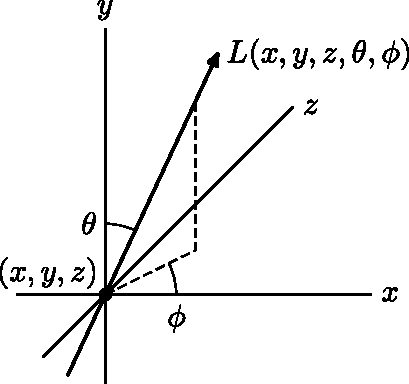
\includegraphics[width=.4\textwidth]{obrazky-figures/plenoptic-function.pdf}
	\caption{Ilustrace plenoptické funkce. Pro zjednodušení není brán v úvahu čas a vlnová délka světla.}
	\label{plenoptic-function}
\end{figure}

Formálně lze plenoptickou funkci definovat jako $P(x, y, z, \theta, \phi, \lambda, t)$, kde
\begin{itemize}
  \item $x, y, z, t$ jsou časoprostorové souřadnice,
  \item $\theta, \phi$ definují prostorový úhel světelného paprsku,
  \item $\lambda$ je vlnová délka světelného paprsku.
\end{itemize}

Jelikož je funkce definovaná v každém bodě v časoprostoru, lze pomocí ní vyjádřit každou scénu, každou fotografii a každý film.
Všechno, co kdy bylo, je a bude viděno.
Naneštěstí toto není v reálném světě možné, proto slouží plenoptická funkce pouze jako idealizovaný koncept.

Tento koncept má však spoustu reálných uplatnění. Příkladem může být třeba první monochromatická fotografie zachycená pomocí dírkové komory.
Tuto fotografii lze definovat jako plenoptickou funkci integrovanou přes viditelné spektrum světla se souřadnicemi ve středu otvoru dírkové komory v čase pořízení a v určitém rozsahu úhlů $\theta, \phi$.
Tyto úhly si lze volně představit jako vertikální a horizontální souřadnice na výsledné fotografii.
Fotografie ve stupních šedi je proto dvourozměrná funkce $F(\theta, \phi)$.

Podobně lze definovat barevnou fotografii jako trojrozměrnou funkci $F(\theta, \phi, \lambda)$, kde oproti monochromatické fotografii není přes vlnovou délku integrováno.
$\lambda$ se tak stává třetím parametrem.
Pokud je k funkci dvourozměrné barevné fotografie přidán parametr $t$, který reprezentuje čas, vznikne čtyřrozměrná funkce $F(\theta, \phi, \lambda, t)$, která reprezentuje video.
Dalším příkladem může být funkce $F(x, y, z, \theta, \phi, \lambda)$ která není parametrizována časem, ale prostorovými souřadnicemi $x, y, z$.
Tato funkce je kompletní holografickou reprezentací zachycené scény v daném čase.

Důležitost plenoptické funkce tedy spočívá v tom, že pomocí jejich řezů lze definovat různé reprezentace zachycené scény.
Jedním z těchto řezů je také 4D světelné pole, kterému se věnuje následující podkapitola.

\section{4D světelné pole}
\label{4D-light-field}
Čtyřrozměrné světelné pole je jedním z mnoha řezů plneoptické funkce.
Tento řez je definován funkcí $F(x, y, \theta, \phi, \lambda)$.
Pozorný čtenář si všimne, že funkce má o jeden rozměr víc, než deklaruje její název.
Jde o vlnovou délku $\lambda$.
Ačkoli se v praxi s barevnými kanály pracuje, v literatuře se pro zjednodušení zanedbává, protože se světelným polem přímo nesouvisí.
Toto zjednodušení je zavedeno i ve zbytku této kapitoly, světelné pole je tedy definováno funkcí $F(x, y, \theta, \phi)$.

Vychází se z předpokladu, že světelné paprsky putující prostorem obvykle nemění svůj směr.
Tím pádem vzniká v plenoptické funkci redundance, protože jeden světelný paprsek se promítne do všech bodů v prostoru $x, y, z$, skrz které tento paprsek prochází.
Tato redundance je podrobněji vykreslena na obrázku \ref{redundance}.
Světelné pole oproti tomu zachycuje paprsek právě jednou, a to v bodě, kde se tento paprsek setkává s rovinou $x, y$.
To demonstruje obrázek \ref{neredundance}.

\begin{figure}[h]
  \centering
  
\includegraphics[width=.4\textwidth]{obrazky-figures/placeholder.pdf}
	\caption{Ukázka redundance v plenoptické funkci.}
	\label{redundance}
\end{figure}

\begin{figure}[h]
  \centering
  
\includegraphics[width=.4\textwidth]{obrazky-figures/placeholder.pdf}
	\caption{Ukázka čtyřrozměrného světelného pole, které řeší redundanci plenoptické funkce.}
	\label{neredundance}
\end{figure}

Čtyřrozmerné světelné pole tedy obsahuje kompletní reprezentaci statické scény pozorované z roviny v prostoru a slouží jako formální aparát pro plenoptické fotografie.

\section{Zachycení plenoptické funkce}
V předchozích podkapitolách jsou popsány řezy plenoptické funkce a jejich souvislost s metodami zachycení scény.
Příkladem je třeba barevná fotografie, kterou lze definovat funkcí $F(\theta, \phi, \lambda)$, kde $\theta, \phi$ jsou prostorové úhly a $\lambda$ je vlnová délka světla.
Jelikož je reálný svět spojitý, je spojitá i plenoptická funkce.
Pokud tedy vychází definice barevné fotografie z plenoptické funkce, znamenalo by to, že scéna je zachycena pro každý úhel pohledu s nekonečnou přesností.

Většina (běžných) fotoaparátů nedokáže vyfotografovat kompletní panormatickou reprezentaci scény, je proto možné funkci zachytit pouze pro určité intervaly hodnot úhlů $\theta, \phi$.
Stejný princip se aplikuje i na další rozměry plenoptické funkce.
Na běžné fotografii například není nutné zachytávat elektromagnetické vlnění mimo viditelné spektrum.
Pro různé profesionální účely naopak můžou existovat kamery, které zachytávají vlnění i mimo viditelné spektrum.

Zároveň není v dnešní době možné dosáhnout nekonečné přesnosti zachycení, funkci je proto pro zachycení potřeba vhodně \textit{vzorkovat}.
Opět platí, že pro každý rozměr plnoptické funkce a pro různé účely zachycení se vzorkování liší.
U běžné fotografie každý ocení vysoké rozlišení (jemné vzorkování úhlů $\theta, \phi$), u videa je navíc důležitá snímková frekvence (vzorkování času $t$).
Oproti tomu například vlnovou délku světla lze často agregovat do trojice hodnot reprezentující červenou, zelenou a modrou barevnou složku (R, G, B) bez viditelné ztráty informace.

Všechny tyto parametry jsou dány výrobcem fotoaparátu, objektivu či jiného zařízení pro zachycení scény.
Stejná pravidla se aplikují i na plenoptické fotografie.

\section{Zachycení plenoptické fotografie}
V technologii plenoptických fotografií se aplikují dva přístupy zachycení, přičemž každý má své výhody, nevýhody a use-cases\footnote{Use-cases -- případy užití.}.

\toto{Tady tím si nejsem moc jistý.}

První z těchto přístupů vzorkuje čtyřrozměrné světelné pole jemně v úhlových dimenzích $\theta, \phi$ na úkor hrubého vzorkování v prostorových dimenzích $x, y$.
Tento přístup je nejčastěji aplikován jako dvourozměrné pole klasických fotoaparátů, které zachycují celou scénu v jeden moment.
Příklad takového pole je demonstrován na obrázku \ref{stanfordArray}.

\label{light-field-capture}
\begin{figure}[h]
  \centering
  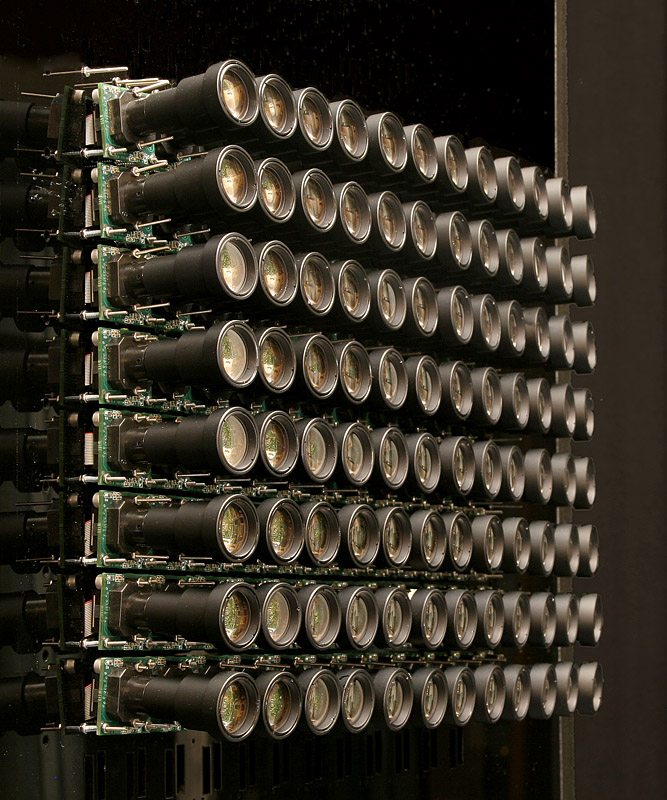
\includegraphics[width=.4\textwidth]{obrazky-figures/stanford-array.jpg}
	\caption{Pole fotoaparátů sestrojené na univerzitě Stanford \cite{stanford-array}.}
	\label{stanfordArray}
\end{figure}

Druhý přístup naopak uplatňuje jemnější vzorkování v dimenzích $x, y$ oproti hrubému vzorkování úhlů $\theta, \phi$.
Tento přístup je vhodný pro menší zařízení, kde všechny pohledy zaznamenává jeden senzor.
Takové zařízení se příliš neliší od klasického fotoaparátu.
Hlavním rozdílem je pole mikročoček umístěné mezi hlavní čočku a světlocitlivý senzor.

\begin{figure}[h]
	\centering
		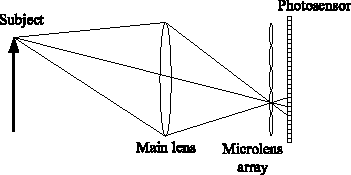
\includegraphics[width=.4\textwidth]{obrazky-figures/pleno-cam.pdf}
		\caption{Princip plenoptického fotoaparátu. Paprsky směřující do fotoaparátu jsou před zachycením na světlocitlivý senzor rozptýleny polem mikročoček.}
		\label{plenoPrincip}
\end{figure}

\section{Formáty pro uložení plenoptických dat}
\label{light-field-formats}
Plenoptická data můžou mít různé formáty a každý formát je vhodný pro jiné využití.
Na jednu stranu je potřeba s těmito daty pracovat rychle a efektivně, na stranu druhou se musí řešit paměťové nároky na uložení těchto dat a s tím související komprese.

Při práci s plenoptickým fotoaparátem se lze nejčastěji setkat s daty v lenslet\footnote{Lenslet -- mikročočka, která je prvkem pole mikročoček \cite{lenslet}.} formátu. Jde o surová data, která jsou zachycena světlocitlivým senzorem v plenoptickém fotoaparátu.
Tato data reflektují rozložení mikročoček ve fotoaparátu.
Pro jejich snažší zpracování jsou k samotné bitmapě přiložena metadata o konstrukci fotoaparátu, který tato data zachytil.
Mimo metadata, která ukládá klasický fotoaparát, se zde zaznamenává zejména informace o velikosti a rozložení mikročoček.

Další alternativou, jak ukládat plenoptické fotografie, je dvourozměrné pole pohledů na tutéž scénu, kde každý pohled reprezentuje snímek scény pod jiným úhlem pozorování.
Tento formát je obvykle výstupem zachycení plenoptické fotografie pomocí dvourozměrného pole fotoaparátů.
Jako metadata jsou v tomto případě uloženy koordináty jednotlivých pohledů, a to buď ve formě vertikálního a horizontálního indexu, nebo lépe také pomocí jednotek reálného světa.
Druhá varianta umožňuje určit měřítko zachycené scény a tím i rozměry objektů, které se ve scéně nacházejí.

Tento formát je vhodný zejména pro kompresi založenou na transformaci a kvantizaci.
Příznivým faktorem pro tuto třídu kompresních algoritmů je silná korelace mezi jednotlivými sousedícími pohledy.
Proto se plenoptické fotografie zachycené plenoptickým fotoaparátem do tohoto formátu často převádí.

Plenoptická data je také možné ukládat jako point cloud\footnote{Point cloud -- množina bodů v prostoru.}.
Tento formát již nezaznamenává paprsky světla zachycené na senzor, nýbrž rekonstruovanou trojrozměrnou scénu, kterou toto světlo reprezentuje.
Point cloud, případně polygonová síť z point cloudu vytvořená, je vhodná pro vykreslení běžnými renderovacími algoritmy.



\chapter{Principy ztrátové komprese využitelné pro plenoptická data}
\label{kompres-teo}
Ztrátová komprese je komprese, při které dochází k nezvratné ztrátě informací, rekonstruovaná data tedy pouze aproximují data původní.
Výhodou dobře implementované ztrátové komprese oproti bezeztrátové kompresi je signifikantní redukce velikosti oproti zanedbatelné degradaci dat.
Díky nedokonalosti lidských smyslů je ztrátová komprese hojně využívaná v oblasti obrazových a zvukových signálů.
U ztrátové komprese je snaha redukovat data, která mají nejmenší význam.

\section{Komprese obrazu}
Nejrozšířenějším standardem pro ztrátovou kompresi se obrazu stal formát JPEG z roku 1992.
Tento formát je založený na diskrétní cosinově transformaci a následné kvantizaci výsledných koeficientů podle citlivosti lidského oka na jednotlivé frekvence v obrazu.

\section{Kompresní řetězec JPEG}
\label{jpeg}

\subsubsection*{Transformace barevného prostoru}

RGB obrázek je vhodné před samotnou transformací převést do vhodného barevného modelu.
K tomuto se vybízí využít model YC\textsubscript{b}C\textsubscript{r}, který barevná data dělí na luminanci Y (jas) a složky chrominance C\textsubscript{b}C\textsubscript{r} (barvy).
Jelikož je lidské oko citvlivé více na jas než na barvu, je možné chromatické složky komprimovat více drasticky bez viditelné ztráty kvality.
Po převodu do vhodného barevného modelu je každý kanál komprimován zvlášť.

\subsubsection*{Dělení do bloků}

Data jednoho komprimovaného kanálu jsou převedeny do bloků velikosti $8\times8$, které jsou následně komprimovány individuálně.
U obrázků, jejichž rozměr není násobkem osmi, vzniká problém krajních bloků.
Obrázek se v tomto případě obvykle rozšíří na násobek osmičky, přičemž existuje několik alternativ, jak vyplnit nově vytvořené krajní pixely.
Nejjednodušší je vyplnit prázdné místo nějakou jednotnou barvou.
Nevýhodou tohoto přístupu je vysoká frekvence, která vzniká skokovým přechodem mezi obrázkem a barvou.
Tento problém dokáže částečně řešit přístup, kdy se redundantní pixely doplní hodnotou krajních pixelů originálního obrázku.
Alernativou může být také zrcadlení původního obrázku nebo jeho opakování (svinutí obrázku do pomyslného torusu).

\subsubsection*{Diskrétní cosinova transformace}

Na každý blok se dále aplikuje diskrétní cosinova transformace.
DCT rozloží blok na DC koeficient -- vlevo nahoře -- reprezentující pouze průměrnou barvu bloku, a AC koeficienty -- všechny ostatní -- reprezentující jednotlivé frekvence.
Jde o transformaci podobnou diskrétní Fourierově transformaci, která produkuje pouze reálné koeficienty.
Diskrétní cosinova transformace je využívána také z důvodu koncentrace nejvíce energie na nejnižších frekvencích, což je z hlediska ztrátové komprese výhodné.

\subsubsection*{Kvantizace}

Na transformované bloky se aplikuje kvantizace.
Kvantizace je jádro ztrátové komprese, v tomto kroku jsou totiž aplikovány ztráty.
Ke kvantizaci se využívá kvantizační matice.
Tato matice byla vytvořena na základě experimentů zkoumajících vlastnosti lidského oka.
Je navržena tak, aby redukovala frekvence, na které je lidské oko nejméně citlivé.
Kvantizace probíhá podělením DCT koeficientů hodnotou v kvantizační matici a následným zaokrouhlením.
Kvantizace má za následek, že většina výsledných koeficientů má hodnotu nula.
Toho je využito zejména v bezeztrátové kompresi, která následuje.

\subsubsection*{Entropické kódování}

Dále je potřeba blok převést do 1D, avšak tak, aby byly kvantizované koeficienty v nejlepším případě seřazeny od největšiho po nejmenší.
K tomu se využívá průchod způsobem cik-cak.
Tento průchod zajišťuje, že DC koeficient bude na jedné straně a AC koeficient s největšimi vertikálními a horizontálnímí frekvencemi bude na straně druhé.

Na DC koeficienty je aplikováno kódování, kdy je od každého DC koeficientu odečten DC koeficient předchozího bloku.
Tyto rozdíly se uloží namísto původních DC koeficientů.

AC koeficienty jsou zakódovány pomocí RLE\footnote{RLE -- Run-length encoding.}.
RLE je provedeno tak, že každý nenulový koeficient v bloku je převeden na dvojici (ZEROES, AMPLITUDE), kde ZEROES je počet nul, které koeficientu předcházely, a AMPLITUDE je samotná hodnota koeficientu.

Toto kódování zahrnuje dvě speciální dvojice.
Tou první je dvojice (0, 0), takzvaný EOB\footnote{EOB -- End-of-block.} -- symbol sloužící jako ukončující značka daného bloku reprezentující zbytek nul na konci.
Kvůli tomu je pro kompresi výhodné řadit koeficienty tak, aby na konci bylo velké množství nul.
Pokud nastane situace, kde je před kódovaným nenulovým koeficientem více než 15 nul, je nutné zavést opatření, která zajistí, že hodnotu počtu nul bude možné uložit do 4 bitů.
Tímto opatřením je dvojice (15, 0), která reprezentuje šestnáct nulových koeficientů za sebou, resp. patnáct předcházejících nul + koeficient s nulovou hodnotou.
Pokud se tedy na vstupu objeví napříkad sedmnáct nul a dvojka, budou výstupem dvojice (15, 0) a (1, 2).

Pro efektivní entropické kódování by bylo vhodné, kdyby měl kódovaný symbol nějakou vhodnou délku.
V předchozím odstavci bylo zmíněno, že ZEROES je hodnota, která se vejde na čtyři bity.
Oproti tomu maximální velikost AMPLITUDE závisí na použité metodě DCT a v obvyklých případech dosahuje až 11 bitů.
Proto metoda JPEG nekóduje dvojice (ZEROES, AMPLITUDE), ale (ZEROES, SIZE), kde SIZE je index nejvyššího jedničkového bitu v absolutní hodnotě kódované amplitudy, ke kterému je přičtena jednička.
Amplituda s hodnotou nula neobsahuje žádný jedničkový bit, hodnota SIZE je v tomto případě 0.
Položka SIZE je bezznaménková a může dosahovat maximální hodnoty 11, k uložení této hodnoty proto vystačí čtyři bity.
Jelikož je každá z těchto hodnot kódovaná na čtyřech bitech, je možné obě tyto hodnoty uložit do jednoto bytu.
Tento byte je symbolem, který je dále entropicky kódován.

Symboly se kódují buď pomocí Huffmanova kódování, nebo pomocí aritmetického kódování.
Huffmanovo kódování je rozšířené pro svoji menší výpočetní náročnost.
K zakódování lze využít již existující huffmanovu tabulku.
Předpočítaná tabulka výrazně šetří čas, ovšem za cenu suboptimální komprese.
Oproti tomu lze huffmanovu tabulku vypočítat speciálně pro pravděpodobnostní rozložení dané kódovaným obrázkem.
Za cenu větší výpočetní náročnosti je proto možné vygenerovat optimální huffmanovu tabulku pro optimální krok bezeztrátové komprese.

V metodě JPEG se obvykle používají zvlášť huffmanovy tabulky pro AC a DC koeficienty a zvlášť také pro luminanci a chrominanci.
Celkem tedy $(AC, DC)\times(luma, chroma)$ čtyři huffmanovy tabulky.
Tyto tabulky jsou uloženy ve výsledném souboru.
Komprese huffmanovy tabulky je možná při použití kanonického huffmanova kódování.

Aritmetické kódování dosahuje lepšího kompresního poměru za cenu větší výpočetní náročnosti při kódování a dekódování.
Proto tato není tak často využívaná v praxi.

Samotná amplituda není entropicky kódovaná, ale ukládá se jen na zakódovaný potřebný počet bitů.
Záporné hodnoty amplitudy se ukládají v jedničkovém doplňku.

\chapter{Implementace kodeku plenoptických fotografií}
\label{lfif-impl}

\chapter{Závěr}
%\label{zaver}




%===============================================================================


  % Kompilace po částech (viz výše, nutno odkomentovat)
  % Compilation piecewise (see above, it is necessary to uncomment it)
  %\subfile{projekt-01-uvod-introduction}
  % ...
  %\subfile{chapters/projekt-05-conclusion}


  % Pouzita literatura / Bibliography
  % ----------------------------------------------
\ifslovak
  \makeatletter
  \def\@openbib@code{\addcontentsline{toc}{chapter}{Literatúra}}
  \makeatother
  \bibliographystyle{bib-styles/slovakiso}
\else
  \ifczech
    \makeatletter
    \def\@openbib@code{\addcontentsline{toc}{chapter}{Literatura}}
    \makeatother
    \bibliographystyle{bib-styles/czechiso}
  \else
    \makeatletter
    \def\@openbib@code{\addcontentsline{toc}{chapter}{Bibliography}}
    \makeatother
    \bibliographystyle{bib-styles/englishiso}
  %  \bibliographystyle{alpha}
  \fi
\fi
  \begin{flushleft}
  \bibliography{xdlaba02-Ztratova-komprese-plenoptickych-fotografii-20-literatura-bibliography}
  \end{flushleft}

  % vynechani stranky v oboustrannem rezimu
  % Skip the page in the two-sided mode
  \iftwoside
    \cleardoublepage
  \fi

  % Prilohy / Appendices
  % ---------------------------------------------
  \appendix
\ifczech
  \renewcommand{\appendixpagename}{Přílohy}
  \renewcommand{\appendixtocname}{Přílohy}
  \renewcommand{\appendixname}{Příloha}
\fi
\ifslovak
  \renewcommand{\appendixpagename}{Prílohy}
  \renewcommand{\appendixtocname}{Prílohy}
  \renewcommand{\appendixname}{Príloha}
\fi
%  \appendixpage

% vynechani stranky v oboustrannem rezimu
% Skip the page in the two-sided mode
%\iftwoside
%  \cleardoublepage
%\fi

\ifslovak
%  \section*{Zoznam príloh}
%  \addcontentsline{toc}{section}{Zoznam príloh}
\else
  \ifczech
%    \section*{Seznam příloh}
%    \addcontentsline{toc}{section}{Seznam příloh}
  \else
%    \section*{List of Appendices}
%    \addcontentsline{toc}{section}{List of Appendices}
  \fi
\fi
  \startcontents[chapters]
  \setlength{\parskip}{0pt}
  % seznam příloh / list of appendices
  % \printcontents[chapters]{l}{0}{\setcounter{tocdepth}{2}}

  \ifODSAZ
    \setlength{\parskip}{0.5\bigskipamount}
  \else
    \setlength{\parskip}{0pt}
  \fi

  % vynechani stranky v oboustrannem rezimu
  \iftwoside
    \cleardoublepage
  \fi

  % Přílohy / Appendices
  %% Tento soubor nahraďte vlastním souborem s přílohami (nadpisy níže jsou pouze pro příklad)
% This file should be replaced with your file with an appendices (headings below are examples only)

% Umístění obsahu paměťového média do příloh je vhodné konzultovat s vedoucím
% Placing of table of contents of the memory media here should be consulted with a supervisor
%\chapter{Obsah přiloženého paměťového média}

%\chapter{Manuál}

%\chapter{Konfigurační soubor} % Configuration file

%\chapter{RelaxNG Schéma konfiguračního souboru} % Scheme of RelaxNG configuration file

%\chapter{Plakát} % poster

\chapter{Jak pracovat s touto šablonou}
\label{jak}

V této příloze je uveden popis jednotlivých částí šablony, po kterém následuje stručný návod, jak s touto šablonou pracovat. Pokud po jejím přečtení k šabloně budete mít nějaké dotazy, připomínky apod., neváhejte a napište na e-mail sablona@fit.vutbr.cz.

\section*{Popis částí šablony}

Po rozbalení šablony naleznete následující soubory a adresáře:
\begin{DESCRIPTION}
  \item [bib-styles] Styly literatury (viz níže). 
  \item [obrazky-figures] Adresář pro Vaše obrázky. Nyní obsahuje placeholder.pdf (tzv. TODO obrázek, který lze použít jako pomůcku při tvorbě technické zprávy), který se s prací neodevzdává. Název adresáře je vhodné zkrátit, aby byl jen ve zvoleném jazyce.
  \item [template-fig] Obrázky šablony (znak VUT).
  \item [fitthesis.cls] Šablona (definice vzhledu).
  \item [Makefile] Makefile pro překlad, počítání normostran, sbalení apod. (viz níže).
  \item [projekt-01-kapitoly-chapters.tex] Soubor pro Váš text (obsah nahraďte).
  \item [projekt-20-literatura-bibliography.bib] Seznam literatury (viz níže).
  \item [projekt-30-prilohy-appendices.tex] Soubor pro přílohy (obsah nahraďte).
  \item [projekt.tex] Hlavní soubor práce -- definice formálních částí.
\end{DESCRIPTION}

Výchozí styl literatury (czechiso) je od Ing. Martínka, přičemž slovenská a anglická verze (slovakiso a englishiso) jsou jeho překlady s drobnými modifikacemi. Oproti normě jsou v~něm určité odlišnosti, ale na FIT je dlouhodobě akceptován. Alternativně můžete využít styl od Ing. Radima Loskota nebo od Ing. Radka Pyšného\footnote{BP Ing. Radka Pyšného \url{http://www.fit.vutbr.cz/study/DP/BP.php?id=7848}}. Alternativní styly obsahují určitá vylepšení, ale zatím nebyly řádně otestovány větším množstvím uživatelů. Lze je považovat za beta verze pro zájemce, kteří svoji práci chtějí mít dokonalou do detailů a neváhají si nastudovat detaily správného formátování citací, aby si mohli ověřit, že je vysázený výsledek v pořádku.

\begin{samepage}
Makefile kromě překladu do PDF nabízí i další funkce:
\begin{itemize}
  \item přejmenování souborů (viz níže),
  \item počítání normostran,
  \item spuštění vlny pro doplnění nezlomitelných mezer,
  \item sbalení výsledku pro odeslání vedoucímu ke kontrole (zkontrolujte, zda sbalí všechny Vámi přidané soubory, a případně doplňte).
\end{itemize}
\end{samepage}

Nezapomeňte, že vlna neřeší všechny nezlomitelné mezery. Vždy je třeba manuální kontrola, zda na konci řádku nezůstalo něco nevhodného -- viz Internetová jazyková příručka\footnote{Internetová jazyková příručka \url{http://prirucka.ujc.cas.cz/?id=880}}.

\paragraph {Pozor na číslování stránek!} Pokud má obsah 2 strany a na 2. jsou jen \uv{Přílohy} a~\uv{Seznam příloh} (ale žádná příloha tam není), z nějakého důvodu se posune číslování stránek o 1 (obsah \uv{nesedí}). Stejný efekt má, když je na 2. či 3. stránce obsahu jen \uv{Literatura} a~je možné, že tohoto problému lze dosáhnout i jinak. Řešení je několik (od~úpravy obsahu, přes nastavení počítadla až po sofistikovanější metody). \textbf{Před odevzdáním proto vždy překontrolujte číslování stran!}


\section*{Doporučený postup práce se šablonou}

\begin{enumerate}
  \item \textbf{Zkontrolujte, zda máte aktuální verzi šablony.} Máte-li šablonu z předchozího roku, na stránkách fakulty již může být novější verze šablony s~aktualizovanými informacemi, opravenými chybami apod.
  \item \textbf{Zvolte si jazyk}, ve kterém budete psát svoji technickou zprávu (česky, slovensky nebo anglicky) a svoji volbu konzultujte s vedoucím práce (nebyla-li dohodnuta předem). Pokud Vámi zvoleným jazykem technické zprávy není čeština, nastavte příslušný parametr šablony v souboru projekt.tex (např.: \verb|documentclass[english]{fitthesis}| a přeložte prohlášení a poděkování do~angličtiny či slovenštiny.
  \item \textbf{Přejmenujte soubory.} Po rozbalení je v šabloně soubor \texttt{projekt.tex}. Pokud jej přeložíte, vznikne PDF s technickou zprávou pojmenované \texttt{projekt.pdf}. Když vedoucímu více studentů pošle \texttt{projekt.pdf} ke kontrole, musí je pracně přejmenovávat. Proto je vždy vhodné tento soubor přejmenovat tak, aby obsahoval Váš login a (případně zkrácené) téma práce. Vyhněte se však použití mezer, diakritiky a speciálních znaků. Vhodný název může být např.: \uv{\texttt{xlogin00-Cisteni-a-extrakce-textu.tex}}. K přejmenování můžete využít i přiložený Makefile:
\begin{verbatim}
make rename NAME=xlogin00-Cisteni-a-extrakce-textu
\end{verbatim}
  \item Vyplňte požadované položky v souboru, který byl původně pojmenován \texttt{projekt.tex}, tedy typ, rok (odevzdání), název práce, svoje jméno, ústav (dle zadání), tituly a~jméno vedoucího, abstrakt, klíčová slova a další formální náležitosti.
  \item Nahraďte obsah souborů s kapitolami práce, literaturou a přílohami obsahem svojí technické zprávy. Jednotlivé přílohy či kapitoly práce může být výhodné uložit do~samostatných souborů -- rozhodnete-li se pro toto řešení, je doporučeno zachovat konvenci pro názvy souborů, přičemž za číslem bude následovat název kapitoly. 
  \item Nepotřebujete-li přílohy, zakomentujte příslušnou část v \texttt{projekt.tex} a příslušný soubor vyprázdněte či smažte. Nesnažte se prosím vymyslet nějakou neúčelnou přílohu jen proto, aby daný soubor bylo čím naplnit. Vhodnou přílohou může být obsah přiloženého paměťového média.
  \item Zadání, které si stáhnete v PDF z IS FIT (odkaz \uv{Zadání pro vložení do práce} či \uv{Thesis assignment}), uložte do souboru \texttt{zadani.pdf} a povolte jeho vložení do práce parametrem šablony v \texttt{projekt.tex} (\verb|documentclass[zadani]{fitthesis}|).
  \item Nechcete-li odkazy tisknout barevně (tedy červený obsah -- bez konzultace s vedoucím nedoporučuji), budete pro tisk vytvářet druhé PDF s tím, že nastavíte parametr šablony pro tisk: (\verb|documentclass[zadani,print]{fitthesis}|). Budete-li tisknout barevně, místo \texttt{print} použijte parametr \texttt{cprint}. Barevné logo se nesmí tisknout černobíle!
  \item Vzor desek, do kterých bude práce vyvázána, si vygenerujte v informačním systému fakulty u zadání. Pro disertační práci lze zapnout parametrem v šabloně \texttt{cover} (více naleznete v souboru \texttt{fitthesis.cls}).
  \item Nezapomeňte, že zdrojové soubory i (obě verze) PDF musíte odevzdat na CD či jiném médiu přiloženém k technické zprávě.
\end{enumerate}

Obsah práce se generuje standardním příkazem \tt \textbackslash tableofcontents \rm (zahrnut v šabloně). Přílohy jsou v něm uvedeny úmyslně.

\subsection*{Pokyny pro oboustranný tisk}
\begin{itemize}
\item \textbf{Oboustranný tisk je doporučeno konzultovat s vedoucím práce.}
\item Je-li práce tištěna oboustranně a její tloušťka je menší než tloušťka desek, nevypadá to dobře.
\item Zapíná se parametrem šablony: \verb|\documentclass[twoside]{fitthesis}|
\item Po vytištění oboustranného listu zkontrolujte, zda je při prosvícení sazební obrazec na obou stranách na stejné pozici. Méně kvalitní tiskárny s duplexní jednotkou mají často posun o 1--3 mm. Toto může být u některých tiskáren řešitelné tak, že vytisknete nejprve liché stránky, pak je dáte do stejného zásobníku a vytisknete sudé.
\item Za titulním listem, obsahem, literaturou, úvodním listem příloh, seznamem příloh a případnými dalšími seznamy je třeba nechat volnou stránku, aby následující část začínala na liché stránce (\textbackslash cleardoublepage).
\item  Konečný výsledek je nutné pečlivě překontrolovat.
\end{itemize}

\subsection*{Styl odstavců}

Odstavce se zarovnávají do bloku a pro jejich formátování existuje více metod. U papírové literatury je častá metoda s~použitím odstavcové zarážky, kdy se u~jednotlivých odstavců textu odsazuje první řádek odstavce asi o~jeden až dva čtverčíky (vždy o~stejnou, předem zvolenou hodnotu), tedy přibližně o~dvě šířky velkého písmene M základního textu. Poslední řádek předchozího odstavce a~první řádek následujícího odstavce se v~takovém případě neoddělují svislou mezerou. Proklad mezi těmito řádky je stejný jako proklad mezi řádky uvnitř odstavce. \cite{fitWeb} 

Další metodou je odsazení odstavců, které je časté u elektronické sazby textů. První řádek odstavce se při této metodě neodsazuje a mezi odstavce se vkládá vertikální mezera o~velikosti 1/2 řádku. Obě metody lze v kvalifikační práci použít, nicméně často je vhodnější druhá z uvedených metod. Metody není vhodné kombinovat.

Jeden z výše uvedených způsobů je v šabloně nastaven jako výchozí, druhý můžete zvolit parametrem šablony \uv{\tt odsaz\rm }.

\subsection*{Užitečné nástroje}
\label{nastroje}

Následující seznam není výčtem všech využitelných nástrojů. Máte-li vyzkoušený osvědčený nástroj, neváhejte jej využít. Pokud však nevíte, který nástroj si zvolit, můžete zvážit některý z následujících:

\begin{description}
	\item[\href{http://miktex.org/download}{MikTeX}] \LaTeX{} pro Windows -- distribuce s jednoduchou instalací a vynikající automatizací stahování balíčků. MikTex obsahuje i vlastní editor, ale spíše doporučuji TeXstudio.
	\item[\href{http://texstudio.sourceforge.net/}{TeXstudio}] Přenositelné opensource GUI pro \LaTeX{}.  Ctrl+klik umožňuje přepínat mezi zdrojovým textem a PDF. Má integrovanou kontrolu pravopisu\footnote{Českou kontrolu pravopisu lze doinstalovat z \url{https://extensions.openoffice.org/de/project/czech-dictionary-pack-ceske-slovniky-cs-cz}}, zvýraznění syntaxe apod. Pro jeho využití je nejprve potřeba nainstalovat MikTeX případně jinou \LaTeX ovou distribuci.
	\item[\href{http://www.winedt.com/}{WinEdt}] Ve Windows je dobrá kombinace WinEdt + MiKTeX. WinEdt je GUI pro Windows, pro jehož využití je nejprve potřeba nainstalovat \href{http://miktex.org/download}{MikTeX} či \href{http://www.tug.org/texlive/}{TeX Live}. 
	\item[\href{http://kile.sourceforge.net/}{Kile}] Editor pro desktopové prostředí KDE (Linux). Umožňuje živé zobrazení náhledu. Pro jeho využití je potřeba mít nainstalovaný \href{http://www.tug.org/texlive/}{TeX Live} a Okular. 
	\item[\href{http://jabref.sourceforge.net/download.php}{JabRef}] Pěkný a jednoduchý program v Javě pro správu souborů s bibliografií (literaturou). Není potřeba se nic učit -- poskytuje jednoduché okno a formulář pro editaci položek.
	\item[\href{https://inkscape.org/en/download/}{InkScape}] Přenositelný opensource editor vektorové grafiky (SVG i PDF). Vynikající nástroj pro tvorbu obrázků do odborného textu. Jeho ovládnutí je obtížnější, ale výsledky stojí za to.
	\item[\href{https://git-scm.com/}{GIT}] Vynikající pro týmovou spolupráci na projektech, ale může výrazně pomoci i jednomu autorovi. Umožňuje jednoduché verzování, zálohování a přenášení mezi více počítači.
	\item[\href{http://www.overleaf.com/}{Overleaf}] Online nástroj pro \LaTeX{}. Přímo zobrazuje náhled a umožňuje jednoduchou spolupráci (vedoucí může průběžně sledovat psaní práce), vyhledávání ve zdrojovém textu kliknutím do PDF, kontrolu pravopisu apod. Zdarma jej však lze využít pouze s určitými omezeními (někomu stačí na disertaci, jiný na ně může narazit i při psaní bakalářské práce) a pro dlouhé texty je pomalejší. Pro vedoucí má FIT licenci a~v~případě, že student narazí na omezení, je s pomocí vedoucího situace řešitelná.
\end{description}

Pozn.: Overleaf nepoužívá Makefile v šabloně -- aby překlad fungoval, je nutné kliknout pravým tlačítkem na \tt projekt.tex \rm a zvolit \uv{Set as Main File}.

\chapter{Psaní anglického textu}
\label{anglicky}
Tato příloha je převzata ze stránek doc. Černockého \cite{CernockyEnglish}.

Spousta lidí píše zprávy k projektům anglicky (a to je dobře!), ale dělá v nich spoustu zbytečných chyb (a to je špatně). Nejsem angličtinář, ale tento jazyk už nějakých pár let používám k psaní, čtení i komunikaci -- tato příloha obsahuje pár důležitých věcí. Pokud chcete napsat práci nebo článek opravdu 100\,\% dobře, nezbude Vám než si najmout rodilého mluvčího (a to by měl by být trochu technicky zdatný a aspoň trochu rozumět tomu, co píšete, ať to neskončí ještě hůř \ldots).

\section*{Obecně}

\begin{itemize}
  \item{Předtím, než budete sami něco psát, si přečtěte pár anglických technických článků a~zkuste si zapamatovat a získat \uv{obecný pocit}, jak se to píše.}
  \item{Používejte vždy korektor pravopisu -- zabudovaný ve Wordu, nebo v OpenOffice, pokud děláte na Linuxu, tak ISPELL a další (většina editorů pro \LaTeX{} má již kontrolu pravopisu integrovanou).}
  \item{Používejte korektor gramatiky. Nevím, jestli je nějaký dostupný na Linuxu, ale ten ve Wordu celkem slušně funguje a pokud Vám něco zelené podtrhne, je tam většinou opravdu chyba. Můžete do něj nakopírovat i zdrojový text pro \LaTeX{}, opravit, a pak uložit opět jako čistý text. Pokud používáte vim, je tam zabudovaný také a zvládne jak překlepy, tak základní gramatiku. V dokumentu \texttt{diplomka.tex} na první řádek napište: 
  \begin{verbatim}
    % vim:spelllang=en_us:spell
  \end{verbatim}
  (případně \texttt{en\_gb} pro OED angličtinu)
  \textit{Poznámka editora:} Existuje i velmi dobrý online nástroj Grammarly\footnote{\url{https://www.grammarly.com/}}, který je v základní verzi zdarma. 
  }
  \item{Online slovníky jsou dobré, ale nepoužívejte je slepě. Většinou dají více variant a ne každá je správně.}
  \item{\begin{samepage}Na vyhledávání a zjištění, co bude asi správné, můžete použít Google. Např.: nevíte, jak se řekne \uv{výhoda tohoto přístupu}. Slovník na seznam.cz dá asi 10 variant. Napište je postupně do vyhledávání na googlu:
  \begin{verbatim}
    "advantage of this approach" 1100000 hits
    "privilege of this approach" 6 hits
    "facility of this approach"  16 hits
  \end{verbatim}
  Neříkám, že je to 100\,\% správně, ale je to určité vodítko. Toto se dá použít i~na~dohledání správných spojek (třeba \uv{among two cases} nebo \uv{between two cases}?)\end{samepage}}
\end{itemize}
       
\section*{SVOMPT a shoda}

Struktura anglické věty je SVOPMT: SUBJECT VERB OBJECT MANNER PLACE TIME a přes to nejede vlak! Není volná jako v češtině. Jinak to je maximálně v nějaké divadelní hře, kde je potřeba něco zdůraznit. Hlavně podmět tam musí vždycky být, na to se často zapomíná, protože v CZ/SK může být zamlčený nebo nevyjádřený. SVOMPT platí i ve vedlejších větách!
\begin{verbatim}
  BAD: We have shown that is faster than the other function. 
  GOOD: We have shown that it is faster than the other function. 
\end{verbatim}

\noindent Shoda podmětu s přísudkem -- zní to šíleně, ale dělá se v tom spousta chyb. 

\begin{verbatim}
  he has 
  the users have 
  people were 
\end{verbatim}

\section*{Členy}

Členy v angličtině jsou noční můra a téměř nikdo z nás je nedává dobře. Základní pravidlo je, že když je něco určitého, musí předtím být \uv{the}. Členy musí být určitě u těchto spojení:
\begin{verbatim}
  the first, the second, ...
  the last
  the most (třetí stupeň přídavných jmen a príslovcí) ...
  the whole 
  the following 
  the figure, the table. 
  the left, the right - on the left pannel, from the left to the right ... 
\end{verbatim}

\noindent Naopak člen NESMÍ být, pokud používáte přesné označení obrázku, kapitoly, atd.
\begin{verbatim}
  in Figure 3.2
  in Chapter 7
  in Table 6.4
\end{verbatim}

\begin{samepage}
\noindent Pozor na \uv{a} vs. \uv{an}, řídí se to podle výslovnosti a ne podle toho, jak je slovo napsané, takže:
\begin{verbatim}
  an HMM
  an XML
  a universal model
  a user
\end{verbatim}
\end{samepage}

\section*{Slovesa}

Pozor na trpné tvary sloves -- u pravidelných je to většinou bez problémů, u nepravidelných často špatně, typicky
\begin{verbatim}
  packet was sent (ne send)
  approach was chosen (ne choosed)
\end{verbatim}
\noindent \ldots vetšinou to opraví korektor pravopisu, ale někdy ne. 

Pozor na časy, občas je v nich pěkný nepořádek. Pokud něco nějak obecně je, přítomný čas. Pokud jste něco udělali, minulý. Pokud to dalo nějaký výsledek a ten výsledek teď existuje a třeba ho nějak diskutujete, přítomný. Nepoužívejte příliš složité časy jako je předpřítomný a vůbec ne předminulý pokud nevíte přesně, co děláte.
\begin{verbatim}
  JFA is a technique that works for everyone in speaker recognition. 
  We implemented it according to Kenny's recipe in \cite{Kenny}. 
  12000 segments from NIST SRE 2006 were processed. When compared 
  with a GMM baseline, the results are completely bad. 
\end{verbatim}

\section*{Délka vět a struktura}

\begin{itemize}
  \item{Pište kratší věty a souvětí, pokud máte něco na 5 řádku, většinou se to nedá číst.}
  \item{Strukturujte věty pomocí čárek (více než v češtině!), hlavně po úvodu věty, po kterém začíná vlastní věta. Někdy se dává čárka i před \uv{and} (na rozdíl od češtiny)}
\end{itemize}
\begin{verbatim}
  In this chapter, we will investigate ... 
  The first technique did not work, the second did not work as well, 
  and the third one also did not work. 
\end{verbatim}

\section*{Specifika technického textu}

Píšete technicky text, proto nepoužívejte zkratky
\begin{verbatim}
  he's
  gonna
  Petr's working on ...
\end{verbatim}
\noindent a podobně. Jediné, které je tolerované, je \uv{doesn't}, ale neuděláte chybu, když napíšete \uv{does not}. 

\begin{samepage}
\noindent V technických textech se spíš používá trpný rod než činný: 
\begin{verbatim}
  BAD: In this chapter, I describe used programming languages. 
  GOOD: In this chapter, used programming languages are described.
\end{verbatim}
\end{samepage}

Pokud už činný použijete, dává se v technických textech spíše \uv{we}, i když na práci děláte sami. \uv{I}, \uv{my}, atd. se používají pouze tam, kde jde o to zdůraznit, že jde o Vaši osobu, tedy třeba v závěru nebo v popisu \uv{originál claims} v disertaci.

\paragraph{Časté chyby ve slovech}

\begin{itemize}
  \item{Pozor na jeho/její, není to it's, ale its }
  \item{Obrázek není picture, ale figure. }
  \item{Spojka \uv{než} je \uv{than}, ne \uv{then} -- bigger than this, smaller than this \ldots hrozně častá chyba! \uv{Then} je pak, potom.}
\end{itemize}


\chapter{Checklist} 
\label{checklist}
Tento checklist byl převzat ze šablony pro kvalifikační práce, která je k dispozici na blogu prof. Herouta \cite{Herout}, který s laskavým dovolením využil nápadu dr. Szökeho%
\footnote{\url{http://blog.igor.szoke.cz/2017/04/predstartovni-priprava-letu-neni.html}}. 

Velká bezpečnost letecké dopravy stojí z části na tom, že lidé kolem letadel mají \textbf{checklisty} na úplně každý, třeba rutinní a dobře zažitý, postup. Jako pilot strpí to, že bude trochu za blbce a opravdu tužtičkou do seznamu úkonů odškrtá dokonale zvládnuté akce, vytiskněte si a odškrtejte před odevzdáním diplomky i vy tento checklist a vyhněte se tak častým chybám, které by mohly mít až fatální následky na výsledné hodnocení Vaší práce.

\subsubsection*{Struktura}
\begin{checklist}
	\item Už ze samotných názvů a struktury kapitol je patrné, že bylo splněno zadání.
	\item V textu se nevyskytuje kapitola, která by měla méně než čtyři strany (kromě úvodu a závěru). Pokud ano, radil(a) jsem se o tom s vedoucím a ten to schválil.
\end{checklist}

\subsubsection*{Obrázky a grafy}
\begin{checklist}
	\item Všechny obrázky a tabulky byly zkontrolovány a jsou poblíž místa, odkud jsou z textu odkazovány, takže nebude problém je najít.
	\item Všechny obrázky a tabulky mají takový popisek, že celý obrázek dává smysl sám o~sobě, bez čtení dalšího textu. Vůbec nevadí, když má popisek několik řádků.
	\item Pokud je obrázek převzatý, tak je to v popisku zmíněno: \uv{Převzato z [X].}
	\item Písmenka ve všech obrázcích používají font podobné velikosti, jako je okolní text (ani výrazně větší, ani výrazně menší).
	\item Grafy a schémata jsou vektorově (tj. v PDF).
	\item Snímky obrazovky nepoužívají ztrátovou kompresi (jsou v PNG).
	\item Všechny obrázky jsou odkázány z textu.
	\item Grafy mají popsané osy (název osy, jednotky, hodnoty) a podle potřeby mřížku.
\end{checklist}

\subsubsection*{Rovnice}
\begin{checklist}
	\item Identifikátory a jejich indexy v rovnicích jsou jednopísmenné (kromě nečastých zvláštních případů jako $t_\mathrm{max}$).
	\item Rovnice jsou číslovány.
	\item Za (nebo vzácně před) rovnicí jsou vysvětleny všechny proměnné a funkce, které zatím vysvětleny nebyly.
\end{checklist}

\subsubsection*{Citace}
\begin{checklist}
    \item \textbf{Všechny použité zdroje jsou citovány.}
	\item Adresy URL odkazující na služby, projekty, zdroje, github apod. jsou odkazovány pomocí \verb|\footnote{\url{...}}|.
    \item Všechny citace používají správné typy.
	\item Citace mají autora, název, vydavatele (název konference), rok vydání.  Když některá nemá, je to dobře zdůvodněný zvláštní případ a vedoucí to odsouhlasil.
\end{checklist}

\subsubsection*{Typografie}
\begin{checklist}
	\item Žádný řádek nepřetéká přes pravý okraj.
	\item Na konci řádku nikde není jednopísmenná předložka (spraví to nedělitelná mezera $\sim$).
	\item Číslo obrázku, tabulky, rovnice, citace není nikde první na novém řádku (spraví to nedělitelná mezera $\sim$).
	\item Před číselným odkazem na poznámku pod čarou nikde není mezera (to jest vždy takto\footnote{příklad poznámky pod čarou}, nikoliv takto \footnote{jiný příklad poznámky pod čarou}).
\end{checklist}

\subsubsection*{Jazyk}
\begin{checklist}
    \item Použil jsem kontrolu pravopisu a v textu nikde nejsou překlepy.
	\item Nechal jsem si text přečíst od (alespoň) jednoho dalšího člověka, který umí dobře česky / anglicky / slovensky.
	\item V práci psané česky nebo slovensky abstrakt zkontroloval někdo, kdo umí opravdu dobře anglicky.
	\item V textu se nikde nepoužívá druhá mluvnická osoba (vy/ty).
	\item Když se v textu vyskytuje první mluvnická osoba (já, my), vždy se popisuje subjektivní záležitost (\textit{rozhodl jsem se}, \textit{navrhl jsem}, \textit{zaměřil jsem se na}, \textit{zjistil jsem} apod.).
	\item V textu se nikde nepoužívají hovorové výrazy.
	\item V českém či slovenském textu se zbytečně nepoužívají anglické výrazy, které mají ustálené české překlady. Např. slovo \textit{defaultní} se nahradí např. slovem \textit{implicitní} nebo \textit{výchozí}.
\end{checklist}

\subsubsection*{Výsledek na datovém médiu, tj. software}
\begin{checklist}
	\item Mám připravené nepřepisovatelné datové médium 
      \begin{itemize}
	  		\item CD-R,
            \item DVD-R,
            \item DVD+R ve formátu ISO9660 (s rozšířením RockRidge a/nebo Jolliet) nebo UDF,
            \item paměťová karta SD (Secure Digital) ve formátu FAT32 nebo exFAT s nastavenou ochranou proti přepisu.
      \end{itemize}
	\item Pokud je výsledek online (služba, aplikace, \dots), URL je viditelně v úvodu a závěru, aby bylo jasné, kde výsledek hledat.
	\item Na médiu nechybí povinné: 
    	\begin{itemize}
    		\item zdrojové kódy (např. Matlab, C/C++,Python, \dots)
            \item knihovny potřebné pro překlad,
            \item přeložené řešení,
            \item PDF s technickou zprávou (je-li pro tisk 2. verze, tak obě),
            \item zdrojový kód zprávy (\LaTeX), 
    	\end{itemize}
        a případně volitelně po dohodě s vedoucím práce
		\begin{itemize}
			\item relevantní (např. testovací) data, 
            \item demonstrační video,
            \item PDF plakátku,
            \item \dots
		\end{itemize}        
	\item Zdrojové kódy jsou refaktorovány, komentovány a označeny hlavičkou s autorstvím, takže se v nich snadno vyzná i někdo další, než sám autor.
    \item Jakákoliv převzatá část zdrojového kódu je řádně citována -- tedy označena úvodním a v případě převzetí více řádků i ukončovacím komentářem. Komentář obsahuje vše, co vyžaduje licence uvedená na webu (vždy je nutné se ji pokusit najít -- např. Stack Overflow\footnote{\url{https://stackoverflow.blog/2009/06/25/attribution-required/}} má striktní pravidla pro citace).
\end{checklist}

\subsubsection*{Odevzdání}

\begin{checklist}
\item Chci práci (na max. 3 roky) utajit? Pokud ano, nejpozději měsíc před termínem odevzdání práce si podám žádost (v IS), ke které přiložím případné stanovisko firmy, jejíž duševní vlastnictví je třeba chránit.
\item Mám splněný minimální počet normostran textu (lze spočítat pomocí Makefile a~odhadem přičíst obrázky). Pokud jsem těsně pod minimem, konzultoval(a) jsem to s~vedoucím.
\item Pokud chci tisknout oboustranně, konzultoval(a) jsem to s~vedoucím a mám správně nastavenou šablonu. Kapitoly začínají na liché stránce.
\item Technickou zprávu mám v deskách z knihařství (min. 1 výtisk, při utajení oba).
\item Za titulním listem práce je zadání (tzn. mám jej stažené z IS a vložené do šablony).
\item V IS jsou abstrakty a klíčová slova.
\item V IS je PDF práce (s klikatelnými odkazy).
\item Oba výtisky práce jsou podepsané.
\item V jednom (při utajení obou) výtisku práce je paměťové médium, na kterém je fixkou napsaný login (fixku na CD lze zapůjčit v knihovně, na Studijním oddělení nebo až při odevzdání).
\end{checklist}


\chapter{\LaTeX pro začátečníky}
\label{latex}

V této kapitole jsou uvedeny některé často využívané balíčky a příkazy pro \LaTeX{}, které mohou být při tvorbě práce potřeba.

\subsection*{Užitečné balíčky}

Studenti při sazbě textu často řeší stejné problémy. Některé z nich lze vyřešit následujícími balíčky pro \LaTeX:

\begin{itemize}
  \item \verb|amsmath| -- rozšířené možnosti sazby rovnic,
  \item \verb|float, afterpage, placeins| -- úprava umístění obrázků/tabulek (specifikátor \texttt{H}),
  \item \verb|fancyvrb, alltt| -- úpravy vlastností prostředí Verbatim, 
  \item \verb|makecell| -- rozšíření možností tabulek,
  \item \verb|pdflscape, rotating| -- natočení stránky o 90 stupňů (pro obrázek či tabulku),
  \item \verb|hyphenat| -- úpravy dělení slov,
  \item \verb|picture, epic, eepic| -- přímé kreslení obrázků.
\end{itemize}

Některé balíčky jsou využity přímo v šabloně (v dolní části souboru \texttt{fitthesis.cls}). Nahlédnutí do jejich dokumentace může být rovněž velmi užitečné.

Sloupec tabulky zarovnaný vlevo s pevnou šířkou je v šabloně definovaný \uv{L} (používá se jako \uv{p}).

Pro odkazování v rámci textu použijte příkaz \verb|\ref{navesti}|. Podle umístění návěští se bude jednat o~číslo kapitoly, podkapitoly, obrázku, tabulky nebo podobného číslovaného prvku). Pokud chcete odkázat stránku práce, použijte příkaz \verb|pageref{navesti}|. Pro citaci literárního odkazu \verb|\cite{identifikator}|. Pro odkazy na rovnice lze použít příkaz \verb|\eqref{navesti}|.

Znak \,--\, (pomlčka) se V \LaTeX u vkládá jako dvě mínus za sebou: -{}-.

\subsection*{Často využívané příkazy pro \LaTeX{}}
\label{sec:Fragments}

Doporučuji nahlédnout do zdrojového textu této podkapitoly a podívat se, jak jsou následující ukázky vysázeny. Ve zdrojovém textu jsou i pomocné komentáře.

% Sloupec zarovnaný vlevo s pevnou šířkou je v šabloně definovaný "L" (používá se jako p)

Příklad tabulky:
\begin{table}[H]
	\vskip6pt
	\caption{Tabulka hodnocení} 
    \vskip6pt
	\centering
	\begin{tabular}{llr}
		\toprule
		\multicolumn{2}{c}{Jméno} \\
		\cmidrule(r){1-2}
		Jméno & Příjmení & Hodnocení \\
		\midrule
		Jan & Novák & $7.5$ \\
		Petr & Novák & $2$ \\
		\bottomrule
	\end{tabular}
	\label{tab:ExampleTable}
\end{table}

% Ohraničení lze upravit dle potřeby:
% http://latex-community.org/forum/viewtopic.php?f=45&t=24323
% http://tex.stackexchange.com/questions/58163/problem-with-multirow-and-table-cell-borders
% http://tex.stackexchange.com/questions/79369/formatting-table-border-and-text-alignment-in-latex-table

\noindent Příklad rovnice:
\begin{equation}
	\cos^3 \theta =\frac{1}{4}\cos\theta+\frac{3}{4}\cos 3\theta
	\label{eq:rovnice2}
\end{equation}
a dvou horizontálně zarovnaných rovnic: % znak & řídí zarovnání
\begin{align} 
    \label{eq:soustava}
	3x &= 6y + 12 \\
	x &= 2y + 4 
\end{align}

Pokud je třeba rovnici citovat v textu, lze použít příkaz \texttt{\\eqref}. Například na rovnici výše lze odkázat~\eqref{eq:rovnice2}. Pokud chcete srovnat číslo rovnic u soustavy, lze použít prostředí \texttt{split}:
\begin{equation} \label{eq:soustavaSrovnana}
\begin{split}
	3x &= 6y + 12 \\
	x &= 2y + 4
\end{split}
\end{equation}

Matematické symboly ($\alpha$) a výrazy lze umístit i do textu $\cos\pi=-1$ a mohou být i~v~poznámce pod čarou%
\footnote{Vzorec v poznámce pod čarou: $\cos\pi=-1$}.

Obrázek~\ref{sirokyObrazek} ukazuje široký obrázek složený z více menších obrázků. Klasický rastrový obrázek se vkládá tak, jak je vidět na obrázku \ref{keepCalm}.

% Využití \begin{figure*} způsobí, že obrázek zabere celou šířku stránky. Takový obrázek dříve mohl být pouze na začátku stránky, případně na konci s využitím balíčku dblfloatfix (případné [h] se ignorovalo a [H] obrázek odstraní). Nové verze LaTeXu už umí i [h].
\begin{figure*}[h]\centering
  \centering
  
\includegraphics[width=\linewidth,height=1.7in]{obrazky-figures/placeholder.pdf}\\[1pt]
  
\includegraphics[width=0.24\linewidth]{obrazky-figures/placeholder.pdf}\hfill
  
\includegraphics[width=0.24\linewidth]{obrazky-figures/placeholder.pdf}\hfill
  
\includegraphics[width=0.24\linewidth]{obrazky-figures/placeholder.pdf}\hfill
  
\includegraphics[width=0.24\linewidth]{obrazky-figures/placeholder.pdf}
  \caption{\textbf{Široký obrázek.} Obrázek může být složen z více menších obrázků. Chcete-li se na tyto dílčí obrázky odkazovat z textu, využijte balíček \texttt{subcaption}.}
  \label{sirokyObrazek}
\end{figure*}

\begin{figure}[hbt]
	\centering
	
\includegraphics[width=0.3\textwidth]{obrazky-figures/keep-calm.png}
	\caption{Dobrý text je špatným textem, který byl několikrát přepsán. Nebojte se prostě něčím začít.}
	\label{keepCalm}
\end{figure}

Další často využívané příkazy naleznete ve zdrojovém textu ukázkového obsahu této šablony.



  % Kompilace po částech (viz výše, nutno odkomentovat)
  % Compilation piecewise (see above, it is necessary to uncomment it)
  %\subfile{xdlaba02-Ztratova-komprese-plenoptickych-fotografii-30-prilohy-appendices}

\end{document}
